\chapter{The \pkg{LiteSolution} Template}
\fancyhead[L]{\,\color{H7}\href{https://github.com/xiamyphys/litesolution}{\faIcon{github}\;\leftmark}}
\fancyhead[R]{\color{H7}\rightmark\,}

\centerline{Xia Mingyu, \href{https://www.hdu.edu.cn}{Hangzhou Dianzi University}}
\yyyymmdddate
\centerline{\mailto{xiamyphys@gmail.com}}
\centerline{\today,\quad Version 1.2a}

This is the document for \pkg{LiteSolution} template, which provides a lite design of the solution of test paper.

Some designs of this template currently only support \textbf{Simplified Chinese (Mainland)}. If necessary, you can change some Chinese characters to the language you want in the \verb|*.cls| file.

\section{Introduction}
\subsection{The purpose of this template}
This template provides a lite and fresh template, and mainly used for typesetting solutions of mid-term or final exam, textbooks and other exercises. This template is developed based on \pkg{ElegantBook} and \href{https://github.com/Azure1210/VividBooK}{\pkg*{VividBooK}}, ported and improved the chapter design module code of \href{https://www.overleaf.com/latex/templates/the-legrand-orange-book-template-english/jtctyfmnpppc}{\pkg*{The Legrand Orange Book}}. I'd like to express my gratitude to the template authors above for their previous work.

If you meet bugs when using this template, or you have better suggestions or ideas, or you want to participate in the development of the template or other templates by me, welcome to contact via email \href{mailto:xiamyphys@gmail.com}{xiamyphys@gmail.com}.

Also, you can join my \textsf\LaTeX{} Template Discussion \href{https://qm.qq.com/q/OnHzbNvVAG}{QQ Group: 760570712} to communicate with me and get the insider preview edition of the template.

\subsection{Loading \pkg{LiteSolution} and its modes}

You should update all the packages to the latest version or switch to portable version instead by implementing the commands 
\begin{verbatim}
    tlmgr update --self --all --reinstall-forcibly-removed
\end{verbatim}

To learn more, please refer to \href{https://tex.stackexchange.com/questions/55437/how-do-i-update-my-tex-distribution}{How do I update my TEX distribution?}

Save the file \verb|litesolution.cls| to your project's root directory, and then create a \verb|.tex| file, just input the command \verb|\documentclass{litesolution}| on the first line.

The template provides 3 modes, \mode{answer}, \mode{mtpro2} and \mode{counter}. Just add the options of the modes you want separately in the square bracket of the command \verb|\documentclass[options]{litesolution}| in your \verb|.tex| file.

\section{Modes of \pkg{LiteSolution}}
\subsection{The \mode{answer} mode}
This mode has two options, \mode{ans} and \mode{noans}, which can show and hide answers respectively. After you choose the \mode{noans}, the contents in the environment \cmd{solution}, the command \cmd{ans} and the answers in the multiple choice questions will all disappear. So the area that originally contained the answer will be replaced by an area of the same blank size. You can generate exams without answers and solutions by enabling \mode{noans}.

\subsection{The \mode{mtpro2} mode}
If you've installed the \emph{Mathtime Pro 2 Lite} font in your computer, then you can use this mode to change the math font.

\subsection{The \mode{counter}}
This mode has two options, \mode{separate} and \mode{continuous}, which can make the page counter between chapters be remaked or continuous.The page numbers between each test question will be continuous when you use the \mode{continuous} mode or the page number of each test question will start from 1 when you use the \mode{separate}.

\section{Commands of \pkg{LiteSolution}}
\subsection{The \cmd{chapterimage} command}
\begin{verbatim}
    \chapterimage{cover1.png}
\end{verbatim}

This command can assign the title background image for each subsequent chapter.

\subsection{The \cmd{chapterfont} command}
\begin{verbatim}
    \chapterfont{PingFang HK}       \chapterfont*{PingFang HK}
\end{verbatim}

This command can assign the title font for each subsequent chapter, if you do not use this command, the title font will be \emph{songti} in Chinese and \emph{Libertinus} in English.

If a star (*) is added after the \verb|\chapterfont|, then \TeX Live will call the font file from the current path, note from the system. And the file in the current path only support the \verb|.ttf| format.

\subsection{The \cmd{ans} command}
This command can underlines the answer and changes the color of the answer to \textcolor{H5}{Blue Sapphire}.

If mode \mode{noans} is enabled, the answer will disappear, leaving only a horizontal line the same width as the answer.

\subsection{The \cmd{solute} command}
\begin{verbatim}
    \solute{3} % create a solution box with the height of 3em.
\end{verbatim}

This command can create a fixable solution box when the mode \mode{noans} is enabled.

\subsection{The \cmd{watermark} command}
\begin{verbatim}
    \watermark{ctanlion.pdf}
\end{verbatim}

This command can add watermark to the document.

\subsection{Other customer commands}
In order to facilitate input, the following commands are scheduled. You can add others in the \verb|*.cls| file as you like.
\vskip1em
\begin{center}
    \begin{tabular}{l|l|l|l|l|l}
        \toprule
        Command & Output & Command & Output & Command & Output\\
        \midrule
        \verb|\titlelogo{#1}{#2}| & Add emoji with link in text & \verb|\point{#1}| & Add score & \verb|\i| & $\mathrm{i}$\\
        \hline
        \verb|\sokka{#1}| & 故本题选择\#1项 & \verb|\d| & $\mathrm{d}$ & \verb|\e| & $\mathrm{e}$\\
        \hline
        \verb|\xSim[#1]{#2}| & $\xSim[r_1\times2]{r_2+r_1}$ & \verb|\ee{#1}| & $\ee{-34}$ & \verb|\mat{#1}^\T| & $\mat{A}^\T$\\
        \hline
        \verb|\rank{#1}| & $\rank{\mat{AB}}$ & \verb|\QED| & \QED & \verb|$5\unit{kg}$| & $5\unit{kg}$\\
        \bottomrule
    \end{tabular}    
\end{center}

\section{Environments of \pkg{LiteSolution}}
\subsection{The \cmd{choice} environment}
There're two variables in this envrionment. The first one is the answer of the choice problem, the second one is the keywords of this choice problem and it's optional.

\begin{tcblisting}{sidebyside}
\begin{choice}{D}[Keywords]
If you want to add choice and keywords.
\begin{tasks}(2) % 2 choices per line
    \task This is choice A  \task This is choice B
    \task This is choice C  \task This is choice D
\end{tasks}
\end{choice}
\end{tcblisting}

\begin{paracol}{2}
    \begin{choice}{D}[Gaussian theory]
        $A$和$B$为两个均匀带电球体,$A$带电荷$+q$,$B$带电荷$-q$,作一与$A$...
        \begin{tasks}(2)
            \task 通过$S$面的电场强度...        \task 通过$S$面的电场强度...
            \task 通过$S$面的电场强度...        \task 通过$S$面的电场强度...
        \end{tasks}
    \end{choice}
    \switchcolumn
    \centering\vfill
    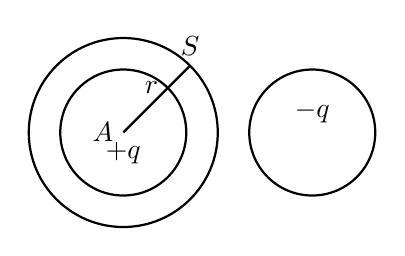
\begin{tikzpicture}
        \draw [thick] (0,0) circle (0.8);
        \draw [thick] (0,0) circle (1.2);
        \draw [thick] (2.4,0) circle (0.8);
        \draw [thick] (0,0)--(0.85,0.85);
        \node [anchor=east] at (0,0) {$A$};
        \node [anchor=north] at (0,0) {$+q$};
        \node [anchor=east] at (0.566,0.566) {$r$};
        \node [anchor=south] at (0.85,0.85) {$S$};
        \node [anchor=south] at (2.4,0) {$-q$};
    \end{tikzpicture}
    \vfill
\end{paracol}
\begin{tcolorbox}
\begin{verbatim}
\begin{paracol}{2}
\begin{choice}{D}[Gaussian theory]
    $A$和$B$为两个均匀带电球体,$A$带电荷$+q$,$B$带电荷$-q$,作一与$A$...
    \begin{tasks}(2)
        \task 通过$S$面的电场强度...        \task 通过$S$面的电场强度...
        \task 通过$S$面的电场强度...        \task 通过$S$面的电场强度...
    \end{tasks}
\end{choice}
\switchcolumn\centering\vfill\tikz{...}\vfill
\end{paracol}
\end{verbatim}
\end{tcolorbox}

\subsection{The \cmd{problem} environment}
Sightly different from the cmd{choice} environment: the two variables are points and keywords, and the question number counter is shared with the multiple-choice question number counter.
\begin{tcblisting}{sidebyside}
    \begin{problem}[Keywords][5]
        If you want to add keywords and points.
    \end{problem}
    \begin{problem}
        If you want to add none.
    \end{problem}
    \begin{problem}[Keywords]
        If you want to add keywords only.
    \end{problem}
    \begin{problem}*[][5]
        If you want to add points only.
    \end{problem}
\end{tcblisting}

\begin{paracol}{2}
\begin{problem}[Gaussian theory \& Field strength][6]
    一均匀带电直导线长为$d$,电荷线密度为$+\lambda$.过导线中点$O$作一半径为$R$($R>\frac{d}{2}$)的球面$S$,$P$为带电直导线的延长线与球面$S$的交点. 则通过该球面的电场强度通量$\Phi_e=$\ans{$\frac{\lambda d}{\varepsilon_0}$},带电直线的延长线与球面交点$P$处的电场强度的大小为\ans{$\frac{\lambda d}{4\pi\varepsilon_0(R^2-d^2/4)}$},方向\ans{沿矢径$\vv{OP}$}.
    \end{problem}
\switchcolumn\centering
\vfill
\begin{tikzpicture}[scale=0.83]
    \draw (0,0) circle (2);
    \draw [thick,->] (-2,0)--(0,0)--(1,1.732);
    \node [anchor=east] at (-2,0) {$P$};
    \filldraw (-2,0) circle (0.05);
    \node [anchor=west] at (0.5,0.866) {$R$};
    \filldraw [pattern=north east lines] (-0.8,-0.1)--(-0.8,0.1)--(0.8,0.1)--(0.8,-0.1)--cycle;
    \draw [thick,|<-] (-0.8,-0.3)--(-0.25,-0.3);
    \draw [thick,|<-] (0.8,-0.3)--(0.25,-0.3);
    \node at (0,-0.3) {$L$};
\end{tikzpicture}
\vfill
\end{paracol}
\begin{tcolorbox}
\begin{verbatim}
\begin{paracol}{2}
    \begin{problem}[Gaussian theory \& Field strength][6]
        一均匀带电直导线长为$d$,电荷线密度为$+\lambda$,过导线中点$O$...
        场强大小\ans{$\frac{\lambda d}{4\pi\varepsilon_0(R^2-d^2/4)}$}...
    \end{problem}
\switchcolumn\centering\vfill\tikz{...}\vfill
\end{paracol}
\end{verbatim}
\end{tcolorbox}

\subsection{The \cmd{note} environment}
\begin{tcblisting}{sidebyside}
\begin{note}
    Please note that...
\end{note}
\end{tcblisting}

\subsection{The \cmd{proof} environment}
\begin{tcblisting}{sidebyside}
\begin{proof}
    Due to \emph{Langrange's Thorem}...
\end{proof}
\end{tcblisting}

If a star (*) is added after the \verb|\begin{solution}|, then the content will follow the 
\begin{tcblisting}{sidebyside}
\begin{proof}*
    Due to \emph{Langrange's Thorem}...
\end{proof}
\end{tcblisting}

\subsection{The \cmd{solution} environment}
\begin{tcblisting}{sidebyside}
\begin{solution}
    This is the answer for the problem.
\end{solution}
\end{tcblisting}

If a star (*) is added after the \verb|\begin{solution}|, then the content will follow the 
\begin{tcblisting}{sidebyside}
\begin{solution}*
    This is the answer for the problem.
\end{solution}
\end{tcblisting}

If mode \mode{noans} is enabled, the solution will disappear, leaving only a blank box with the same height as the solution, and the name of the box will change to \emph{\textcolor{1号色}{\textbf{\faIcon{pen-square} 答题区域}}}.

\section{Known Issues}
\TeX Live will return errors when you enable the mode \mode{noans} and use the \cmd{solution} environment in \cmd{paracol} environment.

\section{Version History}
This template is used to type the mid-term and final exam solutions of \emph{College Physics}. Initially, I used the \href{https://www.ctan.org/pkg/elegantbook}{ElegantBook} template for layout, however, it's no longer be maintained since January 1st, 2023, so I turn to use the \href{https://github.com/Azure1210/VividBooK}{\pkg*{VividBooK}} instead. But this template is too bloated and some functions \& designs need to be redesigned, so I started developing \pkg{LiteSolution}.

\textsf{\bfseries Version 0.1a} was finished developing on 29 June, 2023 and released on \href{https://mp.weixin.qq.com/s/kd4StYk3XybhNQZkAfoY6A}{\faIcon{weixin} WeChat Public Account: 物理问题作} with the name \emph{FreshSolution}. This version redesigned the \cmd{exercise} environment and the \cmd{solution} environment in terms of designs and functions, and improvements have been made to the design of the chapterimage part.

\textsf{\bfseries Version 0.1b} was finished developing on 6 July, 2023 and released on \href{https://www.latexstudio.net/index/details/index/mid/3553.html}{LaTeX Studio} (Xiaoshan, Hangzhou) and \href{http://xhslink.com/YBuuuw}{Xiaohongshu}, where won the favor of many people. This version has added the global option to make the page number be remaked or continuous between chapters, and command \cmd{watermark} has been added in this version.

\textsf{\bfseries Version 1.0a} was finished developing on 15 November, 2023. This version has redesigned the \cmd{chapterimage} part, \cmd{choice} and replaced the \cmd{exercise} environment with the \cmd{problem} environment.

\textsf{\bfseries Version 1.2a} was finished developing on \textcolor{H1}{13 November, 2023}. This version has integrated the chapter design of \href{https://www.ctan.org/pkg/elegantbook}{\pkg*{ElegantBook}} into the star (*) key value of this template \cmd{chapter}. And some commands friendly for matrices typesetting were added in. The command \cmd{chapterfont} was redesigned that it can call the font in the local path or call system font with(out) a star (*) after it. Also, the environment \cmd{proof} was redesigned, and the mode \mode{noans} in this version supports hide the solution box and replace it with a fixable solution box. Today (\textcolor{H1}{2023/12/13}) is \emph{The National public memorial day of Nanjing Massacre}. Hope for world peace.

\newpage
\subsection*{Update Announcements}
\datechange{2023/07/06}{Version 0.1b}
\begin{itemize}
    \item Support page number remaking between chapters.
    \item Added \cmd{watermark} command.
\end{itemize}

\datechange{2023/11/15}{Version 1.0a}
\begin{itemize}
    \item Redesigned the \cmd{chapterimage} part, include the layout and the code.
    \item Redesigned the \cmd{choice} and \cmd{solution} environment, keywords become optional and supports star (*) key. 
    \item Replaced the \cmd{exercise} environment with the \cmd{problem} environment, supports adding only keywords or points.
    \item Added the \cmd{note} environment and some customer commands.
\end{itemize}

\datechange{\today}{Version 1.2a}
\begin{itemize}
    \item Fixed the bug that the gap around the chapter image.
    \item Added some commands for matrices.
    \item Redesigned the \cmd{chapterfont} command.
    \item Redesigned the \cmd{proof} environment.
    \item Supports to adjust the height of solution box when output the exam paper without answer.
    \item Add the \emph{排版规范} in \emph{中文(简体)} after the package document.
    \item Fixed the bug that warnings of the packages \pkg{xeCJK} and \pkg{fontspec}.
\end{itemize}

\subsection*{Future Plans}
\begin{itemize}
    \item Plan to add the \mode{dark} mode to this template to make the text color light while make the page color dark to protect eyesight.
    \item Plan to change the \verb|*.cls| file to a block code design to make it easier for subsequent developers to maintain or modify.
    \item ......
\end{itemize}